\newcommand{\chapter}[2][]{
	\newcommand{\chapname}{#2}
	\begin{flushleft}
		\begin{minipage}[t]{\linewidth}
			
\includegraphics[height=1cm]{hdht-logo.png}
			\hspace{0pt}	
			\sffamily\bfseries\large Bài  21 + Bài 22.
			\begin{flushleft}
				\LARGE\bfseries #1
			\end{flushleft}
		\end{minipage}
	\end{flushleft}
	\vspace{1cm}
	\normalfont\normalsize
}
%\chapter[Momen lực. \\Điều kiện cân bằng tổng quát của vật rắn \\ Thực hành: Tổng hợp lực]{Momen lực. Điều kiện cân bằng tổng quát của vật rắn \\ Thực hành: Tổng hợp lực}
\chapter[Momen lực. \\Điều kiện cân bằng tổng quát của vật rắn ]{Momen lực. Điều kiện cân bằng tổng quát của vật rắn }
\section{Lý thuyết}

\subsection{Momen lực}
Momen lực $M$ đối với một trục quay là đại lượng đặc trưng cho tác dụng làm quay của lực $F$ và được đo bằng tích của lực với cánh tay đòn của nó. Công thức đặc trưng cho momen lực là 
\begin{equation*}
	M = F\cdot d, \label{eq1}
\end{equation*}
trong đó: 
\begin{itemize}
	\item $M$ là momen lực ($\textrm{Nm}$), 
	\item $F$ là lực đang xét ($\textrm{N}$),
	\item $d$ là cánh tay đòn của lực $F$ ($\textrm{m}$).
\end{itemize}

\subsection{Điều kiện cân bằng của một vật có trục quay cố định (Quy tắc momen lực)}
\vspace{-0.5cm}
\subsubsection{Quy tắc momen lực}

Muốn cho một vật có trục quay cố định ở trạng thái cân bằng thì tổng các moment lực có xung hướng làm vật quay theo chiều kim đồng hồ phải bằng tổng các momen lực có xu hướng làm vật quay ngược chiều kim đồng hồ.

\begin{center}
	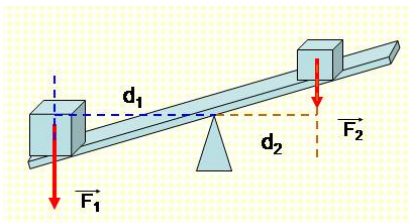
\includegraphics[scale=0.5]{../figs/VN10-PH-21-L-016-2-V2-01.png}
\end{center}

Nếu xét đến hai lực cùng tác dụng vào một vật có trục quay cố định thì vật ở trạng thái cân bằng khi hai lực này tạo ra hai moment lực ngược chiều nhau và độ lớn bằng nhau

\begin{equation*}
	M_1 = M_2,
\end{equation*}
%
hay
%
\begin{equation*}
	F_1\cdot d_1 = F_2\cdot d_2. \label{eq2}
\end{equation*}
%
Nếu xét đến nhiều lực cùng tác dụng vào một vật có trục quay cố định thì vật ở trạng thái cân bằng khi 
%
\begin{align*}
	M_1+M_2+\ldots&= M'_1+M'_2+\ldots\\ 
	\Leftrightarrow\quad F_1\cdot d_1+F_2\cdot d_2 + \ldots &= F'_1\cdot d'_1 + F'_2\cdot d'_2+\ldots
\end{align*}
%
trong đó, các lực $M_1,M_2,\ldots$ tạo ra moment lực cùng chiều với nhau, và ngược chiều với moment lực của các lực $M_1',M_2',\ldots$.
\vspace{0.5cm}
\luuy{Quy tắc momen lực còn được áp dụng cho cả trường hợp một vật không có trục quay cố định nếu như trong một tình huống cụ thể nào đó ở vật xuất hiện trục quay. }
\subsection{Ngẫu lực. Momen ngẫu lực}
\vspace{-0.5cm}
\subsubsection{Ngẫu lực}
Hệ hai lực song song, ngược chiều, có độ lớn bằng nhau và cùng tác dụng vào một vật gọi là ngẫu lực.
\subsubsection{Tác dụng của ngẫu lực đối với một vật rắn}
\textbf{Trường hợp vật không có trục quay cố định}

Dưới tác dụng của ngẫu lực:
\begin{itemize}
	\item  Vật sẽ quay quanh trục đi qua trọng tâm và vuông góc với mặt phẳng chứa ngẫu lực.
	\item Trọng tâm đứng yên. Trục quay đi qua trọng tâm không chịu lực tác dụng.
	\begin{center}
		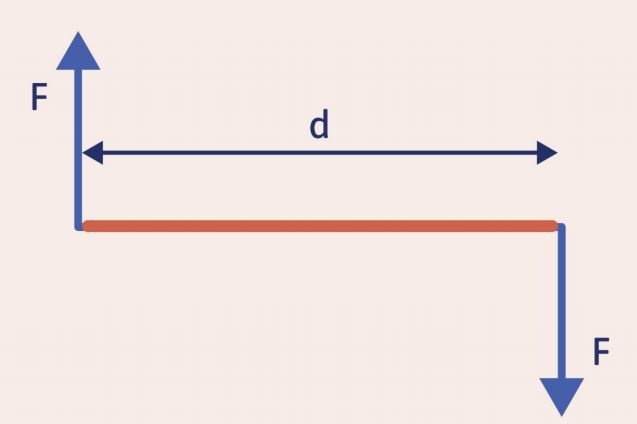
\includegraphics[scale=0.4]{../figs/VN10-PH-25-L-020-1-V2-01.JPG}
	\end{center}	
\end{itemize}
\textbf{Trường hợp vật có trục quay cố định}

Dưới tác dụng của ngẫu lực:
\begin{itemize}
	\item  vật sẽ quay quanh trục cố định của nó. 
	\item Nếu trục quay không đi qua trọng tâm thì trọng tâm sẽ chuyển động tròn xung quanh trục quay. Khi ấy vật có xu hướng chuyển động li tâm nên tác dụng lực vào trục quay.
	\item Khi chế tạo các bộ phận quay của máy móc phải làm cho trục quay đi qua trọng tâm của nó.
	\begin{center}
		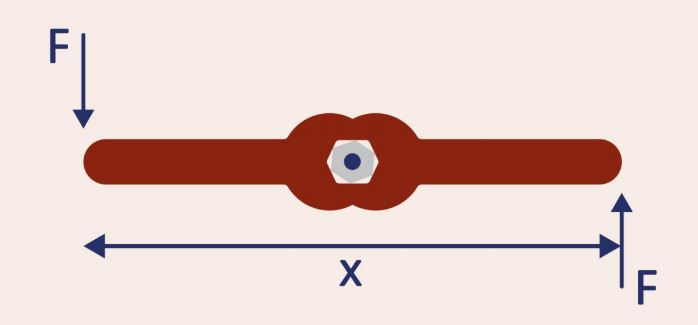
\includegraphics[scale=0.4]{../figs/VN10-PH-25-L-020-1-V2-02.JPG}
	\end{center}
\end{itemize}

\subsubsection{Momen của ngẫu lực}
Đối với các trục quay vuông góc với mặt phẳng chứa ngẫu lực thì momen của ngẫu lực không phụ thuộc vào vị trí trục quay và luôn luôn có giá trị: 
\begin{equation*}
	M=F_1d_1+F_2d_2=F(d_1+d_2)=F\cdot d,
\end{equation*}
trong đó:
\begin{itemize}
	\item $F_1=F_2=F$ là độ lớn của mỗi lực ($\text{N}$);
	\item $d_1+d_2=d$ là khoảng cách giữa hai giá của ngẫu lực và được gọi là cánh tay đòn của ngẫu lực ($\text{m}$);
	\item $M$ là momen của ngẫu lực ($\text{Nm}$).
\end{itemize}
%\subsection{Cách trình bày kết quả trong thực hành tổng hợp lực}
%Trả lời được các câu hỏi sau:
%\begin{itemize}
%	\item Tổng hợp lực là gì? Lực tổng hợp là gì?
%	\item Nêu quy tắc tổng hợp hai lực đồng quy và cách xác định độ lớn của hợp lực.
%\end{itemize}
%\begin{center}
	% Please add the following required packages to your document preamble:
	% \usepackage{multirow}
%	\begin{table}[]
%		\begin{tabular}{|c|l|l|l|l|l|}
%			\hline
%			\textbf{Lần đo n} & \multicolumn{1}{c|}{\textbf{$F_1$ (N)}} & \multicolumn{1}{c|}{\textbf{$F_2$ (N)}} & \multicolumn{1}{c|}{\textbf{Góc $\alpha$}} & \multicolumn{1}{c|}{$F_\text{thực nghiệm}$ (N)} & \multicolumn{1}{c|}{$F_\text{lí thuyết}$ (N)} \\ \hline
%			\textbf{1}        & \multicolumn{1}{c|}{}                   & \multicolumn{1}{c|}{}                   & \multicolumn{1}{c|}{}                      &                                                                              &                                                                            \\ \hline
%			\textbf{2}        &                                         &                                         &                                            &                                                                              &                                                                            \\ \hline
%			\textbf{3}        &                                         &                                         &                                            &                                                                              &                                                                            \\ \hline
%		\end{tabular}
%	\end{table}
%\end{center}
%Kết quả đo:
%\begin{itemize}
%	\item Giá trị trung bình $\bar{F_\text{tn}} = \dfrac{F_{\text{tn1}} + F_{\text{tn2}} + F_{\text{tn3}} + \ldots + F_{\text{tn n}}}{n}$;
%	\item Sai số $\Delta F_{\text{tn n}} = |\bar{F_{\text{tn}}} - F_{\text{tn n}}|$;
%	\item Viết kết quả đo: $F_{\text{tn}}=\bar{F_{\text{tn}}} \pm (\Delta F_{\text{tn}})_\text{max}$.
%\end{itemize}
\section{Mục tiêu bài học - Ví dụ minh họa}
\begin{dang}{Ghi nhớ khái niệm momen lực,\\ công thức tính momen lực}
	\viduii{1}{Đơn vị của momen lực $M = F \cdot d$ là
		\begin{mcq}(4)
			\item $\SI{}{m/s}.$	
			\item $\SI{}{N.m}.$
			\item $\SI{}{kg.m}.$
			\item $\SI{}{N.kg}.$
		\end{mcq}
	}
	{	\begin{center}
			\textbf{Hướng dẫn giải}
		\end{center}
	
	Từ công thức của momen lực		
		\begin{equation*}
			M = F\cdot d, \label{eq1}, 
		\end{equation*}
		trong hệ SI, $F$ có đơn vị là newton (N), $d$ có đơn vị mét (m) nên momen lực có đơn vị newton mét (\SI{}{\newton\meter}).
		
		
		\textbf{Đáp án: B.}
		
	}
	\viduii{1}{Momen lực tác dụng lên vật là đại lượng
		\begin{mcq}
			\item đặc trưng cho tác dụng làm quay vật của lực.
			\item đặc trưng cho tốc độ quay của vật.
			\item để xác định độ lớn của lực tác dụng.
			\item luôn có giá trị dương.
		\end{mcq}		
	}
	{	\begin{center}
			\textbf{Hướng dẫn giải}
		\end{center}
		
		Momen lực $M$ đối với một trục quay là đại lượng đặc trưng cho tác dụng làm quay của lực $F$ và được đo bằng tích của lực với cánh tay đòn của nó.
		
		\textbf{Đáp án: A.}
		
	}
\end{dang}
\begin{dang}{Xác định momen lực và các đại lượng khác\\ trong công thức tính  momen lực}
	\viduii{2}{Một lực có độ lớn $\SI{10}{N}$ tác dụng lên một vật rắn quay quanh trục cố định, biết khoảng cách từ giá của lực đến trục quay là $\SI{20}{cm}.$ Momen của lực tác dụng lên vật có giá trị là	
		\begin{mcq}(4)
			\item $\SI{200}{N.m}.$	
			\item $\SI{20}{N/m}.$
			\item $\SI{2}{N.m}.$
			\item $\SI{0.2}{N/m}.$
		\end{mcq}
	}
	{	\begin{center}
			\textbf{Hướng dẫn giải}
		\end{center}
		
		Momen của lực tác dụng lên vật có giá trị là:
		
		$$M = F \cdot d=\SI{10}{\newton}\cdot\SI{20}{\centi\meter} =\SI{10}{\newton}\cdot\SI{0.2}{\meter}= \SI{2}{N.m}.$$
		
		\textbf{Đáp án: C.}	
		
	}
	\viduii{2}{Một vật rắn chịu tác dụng của lực $F = \SI{20}{N}$ có thể quay quanh trục cố định, khoảng cách từ giá của lực đến trục quay là $\SI{20}{cm}$. Momen của lực $F$ tác dụng lên vật là	
		\begin{mcq}(4)
			\item $\SI{400}{N.m}.$
			\item $\SI{40}{N.m}.$
			\item $\SI{4}{N.m}.$
			\item $\SI{0,4}{N.m}.$	
		\end{mcq}	
	}
	{	\begin{center}
			\textbf{Hướng dẫn giải}
		\end{center}
		
		Momen của lực $F$ tác dụng lên vật có giá trị là:
		
		$$M = F \cdot d = \SI{20}{\newton}\cdot\SI{20}{\centi\meter}=\SI{20}{\newton}\cdot\SI{0.2}{\meter} = \SI{4}{\newton\meter}.$$	
		
		\textbf{Đáp án: C.}	
	}
\end{dang}
\begin{dang}{Ghi nhớ quy tắc momen lực,\\ điều kiện áp dụng quy tắc momen lực}
	\viduii{1}{Phát biểu nào sau đây đúng với quy tắc momen lực?
		\begin{mcq}
			\item Muốn cho một vật có trục quay cố định nằm cân bằng thì tổng momen của các lực có khuynh hướng làm vật quay theo một chiều phải bằng tổng momen của các lực có khuynh hướng làm vật quay theo chiều ngược lại.
			\item Muốn cho một vật có trục quay cố định nằm cân bằng thì tổng momen của các lực phải bằng hằng số.
			\item Muốn cho một vật có trục quay cố định nằm cân bằng thì tổng momen của các lực phải khác không.
			\item Muốn cho một vật có trục quay cố định nằm cân bằng thì tổng momen của các lực phải là một vectơ có giá đi qua trục quay.
		\end{mcq}	
		
	}
	{	\begin{center}
			\textbf{Hướng dẫn giải}
		\end{center}
		
		Muốn cho một vật có trục quay cố định nằm cân bằng thì tổng momen của các lực có khuynh hướng làm vật quay theo một chiều phải bằng tổng momen của các lực có khuynh hướng làm vật quay theo chiều ngược lại.
		
		\textbf{Đáp án: A.}
		
	}
	\viduii{1}{Điều kiện cân bằng của một chất điểm có trục quay cố định còn gọi là
		\begin{mcq}
			\item quy tắc hợp lực đồng quy.
			\item quy tắc hợp lực song song.
			\item quy tắc hình bình hành.
			\item quy tắc momen lực.
		\end{mcq}		
	}
	{	\begin{center}
			\textbf{Hướng dẫn giải}
		\end{center}
		
		Điều kiện cân bằng của một chất điểm có trục quay cố định còn gọi là quy tắc momen lực.
		
		\textbf{Đáp án: D.}
	}
\end{dang}
\begin{dang}{Thực hiện áp dụng quy tắc momen lực để giải bài tập}
	\viduii{2}{Một người dùng búa để nhổ một chiếc đinh, khi người đó tác dụng một lực $\SI{50}{N}$ vào đầu búa thì đinh bắt chuyển động. Biết cánh tay đòn của lực tác dụng của người đó là $\SI{20}{cm}$ và cánh tay đòn của lực ma sát giữa đinh và gỗ là $\SI{2}{cm}$. Hãy tính lực ma sát do gỗ tác dụng vào đinh.	
	}
	{	\begin{center}
			\textbf{Hướng dẫn giải}
		\end{center}
		
		Gọi 
		\begin{itemize}
			\item $M_1$ và $M_2$ là momen lực do tay người và lực cản của gỗ tác dụng lên búa ,
			\item $F_1=\SI{50}{\newton}$ là lực do tay người tác dụng vào đầu búa,
			\item $F_2$ là lực ma sát của gỗ tác dụng lên đinh, 
			\item  $d_1=\SI{20}{cm}$ là cánh tay đòn từ tay người đến trục quay, 
			\item  $d_2=\SI{2}{cm}$ là cánh tay đòn từ đinh đến trục quay. 
		\end{itemize}
		
		Khi đinh bắt đầu chuyển động, câu búa đang ở trạng thái cân bằng, nên ta áp dụng quy tắc momen lực
		
		$$M_1=M_2 \Rightarrow F_1\cdot d_1 = F_2\cdot d_2$$
		
		Lực ma sát do gỗ tác dụng vào đinh 
		
		$$F_2=\dfrac{d_1}{d_2}\cdot F_1=\dfrac{\SI{20}{\centi\meter}}{\SI{2}{\centi\meter}}\cdot\SI{50}{\newton}=\SI{500}{N}.$$
		
		Vậy lực cản do miếng gỗ tác dụng lên cây đinh lúc đó là $F_2=\SI{500}{N}$.
	}
	\viduii{3}{Một thanh AB có chiều dài $\SI{7,5}{m}$ có trọng lượng $\SI{200}{N}$ có trọng tâm G cách đầu A một đoạn $\SI{2}{m}$. Thanh có thể quay xung quanh một trục đi qua O cách A $ \SI{2,5}{m}$. Để thanh cân bằng phải tác dụng vào đầu B một lực $F$ có độ lớn bằng bao nhiêu?		
	}
	{	\begin{center}
			\textbf{Hướng dẫn giải}
		\end{center}
		
		Gọi: 
		\begin{itemize}
			\item $M_1$ và $M_2$ là momen của trọng lực và của lực  tác dụng vào đầu B của thanh,
			\item $F$ là lực tác dụng lên thanh AB tại B, 
			\item  $d_1=\text{OA}-\text{GA}=\SI{0.5}{\meter}$ là cánh tay đòn từ điểm G đến O, 
			\item  $d_2=\text{AB}-\text{OA}=\SI{5}{\meter}$ là cánh tay đòn từ điểm B đến O.
		\end{itemize}
		
		Để AB cân bằng, quy tắc momen lực đòi hỏi 
		
		$$M_1=M_2 \quad \Rightarrow\quad P\cdot d_1 = F\cdot d_2.$$
		
		Vậy để thanh AB cân bằng, lực tác dụng vào điểm B với độ lớn
		
		$$F= \dfrac{d_1}{d_2}\cdot P=\dfrac{\SI{0.5}{\meter}}{\SI{5}{\meter}}\cdot\SI{200}{\newton}=\SI{20}{N}.$$
		
	}
	\viduii{3}{Một thanh gỗ dài $\SI{1,8}{m}$ nặng $\SI{30}{kg}$, một đầu được gắn vào trần nhà nhờ một bản lề, đầu còn lại được buộc vào một sợi dây và gắn vào trần nhà sao cho phương của sợi dây thẳng đứng và giữ cho tấm gỗ nằm nghiêng hợp với trần nhà nằm ngang một góc $45^{\circ}$. Biết trọng tâm của thanh gỗ cách đầu gắn sợi dây $\SI{60}{cm}$. Tính lực căng của sợi dây, lấy $g=\SI[parse-numbers=false]{10}{m/s^2}$.
		\begin{center}
			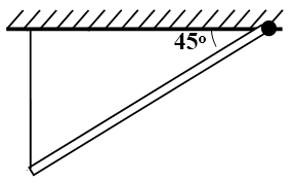
\includegraphics[scale=0.7]{../figs/VN10-PH-21-L-016-2-V2-02.png}
		\end{center}	
		
	}
	{	\begin{center}
			\textbf{Hướng dẫn giải}
		\end{center}
		
		Đầu tiên, ta quy định các đại lượng trong bài toán và xác định cánh tay đòn như sau: 
		\begin{itemize}
			\item $T$ là lực căng của sợi dây tác dụng lên điểm A trên tấm gỗ, 
			\item $P=m\cdot g= \SI{30}{kg} = \SI{300}{N}$ là trọng lực tác dụng lên tấm gỗ tại trọng tâm G, 
			\item $\alpha = 45^{\circ}$ là góc hợp bởi tấm gỗ và trần nhà, 
			\item $d$ là khoảng cách từ điểm G đến trục quay O,
			\item $d'$ là khoảng cách từ điểm treo của dây đến trục quay O,
			\item $l=\SI{1,8}{m}$ là chiều dài của thanh gỗ. 
		\end{itemize}
		%--------------------------------%
		\begin{center}
			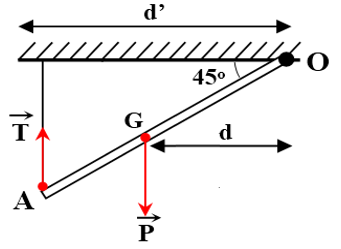
\includegraphics[scale=0.7]{../figs/VN10-PH-21-L-016-2-V2-03.png}
		\end{center}
		Cánh tay đòn của trọng lực
		
		$$d=\text{OG}\cdot\alpha=(\text{0A}-\text{GA})\cos\alpha=(\SI{1.8}{\meter}-\SI{0.6}{\meter})\cos\SI{45}{\degree}=\SI{1.2}{\meter}\cdot\cos\SI{45}{\degree}$$
		
		Cánh tay đòn tương ứng với lực căng dây là
		
		$$d' = \textrm{OA}\cdot\cos\alpha=\SI{1.8}{\meter}\cdot \cos 45^{\circ} .$$
		
		Áp dụng quy tắc momen lực
		\begin{align*}
			T\cdot d' &= P\cdot d\\
			\Rightarrow
			T&=\dfrac{d}{ d'}\cdot P\\
			&=\dfrac{\SI{1.2}{\meter}\cdot\cos\SI{45}{\degree}}{\SI{1.8}{\meter}\cdot\cos\SI{45}{\degree}}\cdot\SI{300}{\newton}\\&=\SI{200}{N}.
		\end{align*}
		Vậy lực căng dây là $T=\SI{200}{N}$. 
	}
	\viduii{3}{Thanh OA có khối lượng không đáng kể, có chiều dài $\SI{20}{cm}$, quay dễ dàng quanh trục nằm ngang O. Một lò xo gắn vào điểm giữa C. Người ta tác dụng vào đầu A của thanh một lực $F=\SI{20}{N}$ hướng thẳng đứng xuống dưới. Khi thanh ở trạng thái cân bằng, lò xo có hướng vuông góc với OA, và OA hợp với đường thẳng nằm ngang một góc $\alpha=30^{\circ}$. Tìm phản lực N của lò xo lên thanh. 
		\begin{center}
			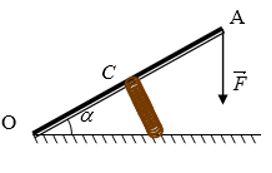
\includegraphics[scale=0.8]{../figs/VN10-PH-21-L-016-2-V2-04.png}
		\end{center}		
	}
	{	\begin{center}
			\textbf{Hướng dẫn giải}
		\end{center}
		
		Các lực tác dụng lên thanh được biểu diễn như hình vẽ. 
		\begin{center}
			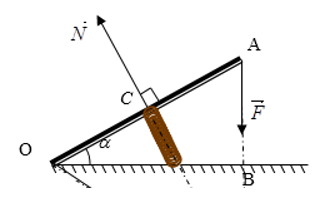
\includegraphics[scale=0.8]{../figs/VN10-PH-21-L-016-2-V2-05.png}
		\end{center}
				
		Do phản lực $N$ vuông góc với thanh nên cánh tay đòn của phản lực $N$ đối với trục quay qua O là 
		$$\textrm{OC} = \dfrac{1}{2}\cdot \textrm{OA},$$
		
		Cánh tay đòn tương ứng với lực $F$ là
		$$\textrm{OB} = \textrm{OA}\cdot \cos\alpha.$$
		
		
		Áp dụng quy tắc momen lực
		
		\begin{alignat*}{4}
			&M_F&=&M_N\\
			\Rightarrow\quad& F\cdot \textrm{OB} &=& N\cdot \textrm{OC}\\
			\Rightarrow\quad& N  &=& \dfrac{F\cdot \textrm{OB}}{\textrm{OC}}\\
			&&=&
			\dfrac{F\cdot \textrm{OA}\cdot \cos\alpha}{\textrm{OA}/2}\\
			&&=&2 F\cos\alpha \\
			&&=& \SI[parse-numbers=false]{20\sqrt{3}}{N}.
		\end{alignat*}
		%%%%
		Vậy phản lực tác dụng lên thanh có độ lớn là $N=\xsi{20\sqrt{3}}{N}$
		
	}
	
\end{dang}
\begin{dang}{Ghi nhớ khái niệm ngẫu lực,\\ đặc điểm ngẫu lực}
	\viduii{1}{Ngẫu lực là gì?
		\begin{mcq}
			\item Là hệ hai lực song song, cùng chiều.
			\item Là hệ hai lực song song, ngược chiều.
			\item Là hệ hai lực song song, cùng chiều có độ lớn bằng nhau và cùng tác dụng vào một vật.
			\item Là hệ hai lực song song, ngược chiều có độ lớn bằng nhau và cùng tác dụng vào một vật.
		\end{mcq}
	}
	{	\begin{center}
			\textbf{Hướng dẫn giải}
		\end{center}
		
		Ngẫu lực là hệ hai lực song song, ngược chiều có độ lớn bằng nhau và cùng tác dụng vào một vật.
		
		\textbf{Đáp án: D.}
	}
	\viduii{1}{Chọn phát biểu sai	
		\begin{mcq}
			\item Tác dụng của ngẫu lực vào một vật làm cho vật quay và tịnh tiến.
			\item Ngẫu lực là hệ hai lực song song, cùng chiều có độ lớn bằng nhau và cùng tác dụng vào một vật.
			\item Đơn vị của ngẫu lực là $\SI{}{N\cdot m}$.
			\item Cả A và B sai.
		\end{mcq}	
	}
	{	\begin{center}
			\textbf{Hướng dẫn giải}
		\end{center}
		
		Ngẫu lực là hệ hai lực song song, \textit{ngược chiều} có độ lớn bằng nhau và cùng tác dụng vào một vật $\rightarrow$ đáp án B sai 
		
		Do hai lực bằng nhau nên hợp lực tác dụng lên vật bằng không, do đó không có tác dụng tịnh tiến vật mà chỉ có tác dụng làm quay vật $\rightarrow$ đáp án A sai. 
		
		Đơn vị của ngẫu lực là newton, còn đơn vị của momen ngẫu lực mới là newton mét ($\SI{}{N\cdot m}$) $\rightarrow$ đáp án C sai.
		
		\textbf{Đáp án: D.}
	}
\end{dang}
\begin{dang}{Áp dụng công thức tính momen ngẫu lực}
%	\viduii{3}{Hai người khiêng một vật nặng $100\ \textrm{kg}$ bằng một đòn gánh dài $1\ \textrm{m}$, biết điểm treo vật cách vai người thứ nhất $60\ \text{cm}$. Tính lực tác dụng lên vai của mỗi người, lấy $g=\SI{10}{\meter/\second^2}$, bỏ qua khối lượng của đòn gánh.	
%	}
%	{	\begin{center}
%			\textbf{Hướng dẫn giải}
%		\end{center}
		
%		Lực tác dụng lên hai người khiêng sẽ bằng trọng lực của vật: 
		
%		$$P=F=m \cdot g=\SI{1000}{\newton}. $$
		
%		Khoảng cách treo vật cách vai người thứ nhất $d_1=\SI{0,6}{\meter}$, $d_2=\SI{0,4}{\meter}$.
		
%		Lực tác dụng lên mỗi vai bằng:
		
%		$$F=F_1+F_2=\SI{1000}{N}.$$ 
		
%		Áp dụng công thức momen của ngẫu lực:
		
%		$$F_1d_1=F_2d_2. $$
		
%		Từ biểu thức của lực tác dụng lên vai và công thức momen ngẫu lực 
		
%		$$F_1=\SI{400}{N};\ F_2=\SI{600}{N}$$
%	}
	\viduii{2}{Hai lực của một ngẫu lực có độ lớn $F= \SI{5,0}{\newton}$. Cánh tay đòn của ngẫu lực $d=\SI{20}{cm}$. Momen của ngẫu lực này là 
		\begin{mcq}(4)
			\item $\SI{10,0}{Nm}$.
			\item $\SI{2,0}{Nm}.$
			\item $\SI{0,5}{Nm}.$
			\item $\SI{1,0}{Nm}.$
		\end{mcq}		
	}
	{	\begin{center}
			\textbf{Hướng dẫn giải}
		\end{center}
		
		Momen ngẫu lực này là:
		
		$$M=F \cdot d= \SI{1,0}{Nm}.$$
		
		\textbf{Đáp án: D.}
	}
\end{dang}